\documentclass[tikz]{standalone}
\usepackage[utf8]{inputenc}
\usepackage{tikz}
\usepackage{xcolor}
\usepackage{xcolor}
\usepackage{scalerel}
\usepackage{graphicx}
\usetikzlibrary{decorations.pathreplacing,calligraphy}
\usepackage{amsmath,amssymb,amsfonts}
\usepackage{dsfont}
\usetikzlibrary{matrix}

\definecolor{MyGreen}{RGB}{34,139,34}

\begin{document}

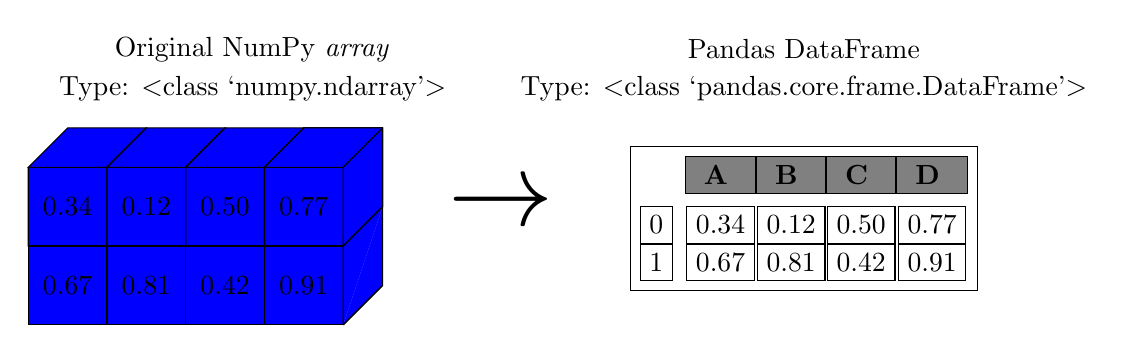
\begin{tikzpicture}[z={(0.5,0.5)}]

\node[align=left] at (3.85,-0.5) {\text{{Original NumPy \textit{array}}}};
\node[align=left] at (3.85,-1) {\text{Type: $<$class \lq numpy.ndarray\rq$>$}};
\def\cubesAmount{3}
\foreach \i in {1,...,\cubesAmount}{
    \draw[fill = blue] (\i,-3,0) rectangle +(1,1,0) -- ++(0,1,0) -- ++(0,0,1) -- ++(1,0,0) edge +(0,0,-1)  -- ++(0,0,-1);
    %\draw[fill = blue] (\i,-6,0) rectangle +(1,1,0) -- ++(0,1,0) -- ++(0,0,1) -- ++(1,0,0) edge +(0,0,-1)  -- ++(0,0,-1);
    \draw[fill = blue] (4,-3,0) rectangle +(1,1,0) -- ++(0,1,0) -- ++(0,0,1) -- ++(1,0,0) edge +(0,0,-1) -- ++(0,-1,0) -- ++(0,0,-1);
    \draw[fill = blue] (\i,-4,0) rectangle +(1,1,0) -- ++(0,1,0);
      \draw[fill = blue] (4,-4,0) rectangle +(1,1,0) -- ++(0,1,0);
    %\draw[fill = blue] (\i,-5,0) rectangle +(1,1,0) -- ++(0,1,0);
   %\draw[fill = blue] (7,-2,0) edge +(0,0,-1) -- ++(0,-1,0) -- ++(0,0,-1);
    %\draw[fill = blue] (\i,-7,0) rectangle +(1,1,0) -- ++(0,1,0) ;
    \ifnum\i<\cubesAmount
       ;
    \fi
}

\draw[fill = blue] (5.5, -2.5,0) edge +(0,0,-1) -- ++(0,-1,0) -- ++(0,0,-1);
\draw[fill = blue, rotate=180] (-5.001, 4.001,0) edge +(0,0,-1) -- ++(0,-1,0) -- ++(0,0,-1);


%\draw[fill = blue] (6.5, -3.5,0) edge +(0,0,-1) -- ++(0,-1,0) -- ++(0,0,-1);
%\draw[fill = blue, rotate=180] (-6.001, 5.001,0) edge +(0,0,-1) -- ++(0,-1,0) -- ++(0,0,-1);

%\draw[fill = blue] (6.5, -5.5,0) edge +(0,0,-1) -- ++(0,-1,0) -- ++(0,0,-1);
%\draw[fill = blue, rotate=180] (-6.001, 7.001,0) edge +(0,0,-1) -- ++(0,-1,0) -- ++(0,0,-1);

%\draw[fill = blue] (6.5, -4.5,0) edge +(0,0,-1) -- ++(0,-1,0) -- ++(0,0,-1);
%\draw[fill = blue, rotate=180] (-6.001, 6.001,0) edge +(0,0,-1) -- ++(0,-1,0) -- ++(0,0,-1);

\node[align=left] at (7,-2.5) {\resizebox{0.11\hsize}{!}{$\rightarrow$}};

\node[align=left] at (1.5,-2.5) {0.34};
\node[align=left] at (2.5,-2.5) {0.12};
\node[align=left] at (3.5,-2.5) {0.50};
\node[align=left] at (4.5,-2.5) {0.77};

\node[align=left] at (1.5,-3.5) {0.67};
\node[align=left] at (2.5,-3.5) {0.81};
\node[align=left] at (3.5,-3.5) {0.42};
\node[align=left] at (4.5,-3.5) {0.91};


\node[align=left] at (10.85,-0.5) {\text{{Pandas {\fontfamily{cmt}\selectfont DataFrame}}}};
\node[align=left] at (10.85,-1) {\text{Type: $<$class \lq pandas.core.frame.DataFrame\rq$>$}};
  \matrix at (10.85,-2.65) [draw,nodes=draw,column sep=1mm]
  {
    &[0.5mm] \node[fill=gray] { \ \textbf{A} \ \ }; &[-1mm] \node[fill=gray] {\ \textbf{B} \ \ };&[-1mm] \node[fill=gray]  {\ \textbf{C} \ \ };&[-1mm] \node[fill=gray]  {\ \textbf{D} \ \ }; \\ [1.5mm]
    \node {0}; &[0.5mm] \node{0.34}; &[-1mm] \node {0.12};&[-1mm] \node {0.50};&[-1mm] \node {0.77}; \\
    \node {1}; &      \node{0.67}; &       \node {0.81};&       \node {0.42};&       \node {0.91}; \\
  };

\end{tikzpicture}






\end{document}


